\subsection{Five tasks with instructions: the certified switch}
\label{sec:five}

\begin{table}[t]
  \caption{Five-task sequence, original instructions (T5-base, 10 epochs per task; re-test against
  all reference answers). Score right after learning: average score of each task right after it was learned. AP:
  average score after the last task. Answers changed: test inputs of the first four
  tasks whose answer at the end differs from the answer given right after their task was learned.
  Certified: test inputs inside a zone.
  Scores are means over \FiveCertSeeds{} seeds, with the lowest and the highest seed in brackets; counts are summed over the seeds.}
  \label{tab:fivemain}
  \centering
  \small
  \setlength{\tabcolsep}{4pt}
  \begin{tabular}{lccccc}
    \toprule
    Method & \shortstack[c]{Score\\right after\\learning $\uparrow$} & \shortstack[c]{Final\\score $\uparrow$} & \shortstack[c]{Forgetting\\(points) $\downarrow$} & \shortstack[c]{Answers\\changed $\downarrow$} & Certified inputs \\
    \midrule
    \cert{} (ours) & 79.74 {\scriptsize(79.2--80.8)} & 79.74 {\scriptsize(79.2--80.8)} & 0.00 & 0 of 1{,}200 & 1{,}500 of 1{,}500 \\
    \nearest{} & 79.74 {\scriptsize(79.2--80.8)} & 79.74 {\scriptsize(79.2--80.8)} & 0.00 & 0 of 1{,}200 &  \\
    \centre{} & 79.74 {\scriptsize(79.2--80.8)} & 79.74 {\scriptsize(79.2--80.8)} & 0.00 & 0 of 1{,}200 &  \\
    \keyswitch{} & 79.74 {\scriptsize(79.2--80.8)} & 79.74 {\scriptsize(79.2--80.8)} & 0.00 & 0 of 1{,}200 &  \\
    \plain{} & 79.74 {\scriptsize(79.2--80.8)} & 36.08 {\scriptsize(32.3--39.5)} & 54.58 {\scriptsize(51.6--58.6)} & 994 of 1{,}200 &  \\
    \midrule
    InfLoRA & 60.02 {\scriptsize(56.6--63.3)} & 62.93 {\scriptsize(59.0--65.4)} & $-$3.14 {\scriptsize($-$5.3 to $-$1.7)} & 370 of 1{,}200 &  \\
    GainLoRA & 61.42 {\scriptsize(59.1--64.4)} & 61.96 {\scriptsize(60.9--63.9)} & $-$0.51 {\scriptsize($-$2.6 to 0.7)} & 65 of 1{,}200 &  \\
    \bottomrule
\end{tabular}

\end{table}

\begin{figure}[t]
  \centering
  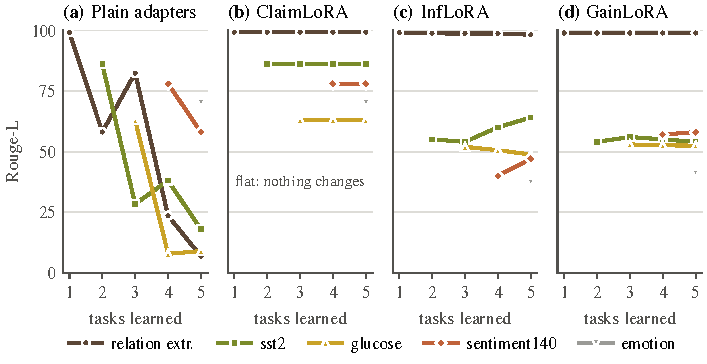
\includegraphics[width=\linewidth]{figures/five_tracks}
  \caption{Score of each of the five tasks as further tasks are learned (seed 42, original
  instructions). With plain adapters every task falls as soon as the next one is learned. With the
  certified switch the same adapters give flat lines. The two published methods are flat as well,
  at a lower level.}
  \label{fig:fivetracks}
\end{figure}

Table~\ref{tab:fivemain} and Figure~\ref{fig:fivetracks} give the result with instructions.

\paragraph{The certified switch keeps every answer.} With the certified switch the average score after the fifth task equals the
average score right after learning, \FiveCertAP{} Rouge-L. Forgetting is \FiveCertFT{}, and none of
the \FiveCertCompared{} answers to the test inputs of the first four tasks differs from the answer
that was given when the task had just been learned. All \FiveCertInputsOne{} test inputs lie inside
their own zone, as Proposition~\ref{prop:own} says they must, and no training input of a later
task lay inside an older zone (\FiveCertBlocked{} of \FiveCertTrainInputs{}). The outcome is therefore not an
observation about these runs but a consequence of Theorem~\ref{thm:writeonce}, and the experiment
confirms that the implementation does what the theorem describes. With the original instructions
\nearest{}, \centre{} and \keyswitch{} choose the same routes and give the same numbers.

\paragraph{The same adapters without a switch lose most of what they learned.} The rows from \cert{} to \plain{} use the same trained adapters; only the switches
differ. With all adapters on, the average falls from \FivePlainLearned{} right after learning to
\FivePlainAP{} at the end, forgetting is \FivePlainFT{} points, and \FivePlainChanged{} of
\FivePlainCompared{} answers change. Relation extraction, the first task, falls from
\FivePlainRelationLearned{} to \FivePlainRelationEnd{} on average over seeds (to 6.8 in the seed of
Figure~\ref{fig:fivetracks}a); only the task that was learned last is intact.

\paragraph{The published methods learned less here.} InfLoRA and GainLoRA have forgetting scores near zero on these five tasks
(\FiveInfFT{} and \FiveGainFT{} points; a
negative value means that old tasks improved on average while later ones were learned), though \FiveInfChanged{} and \FiveGainChanged{} of \FiveInfCompared{} answers change. Their curves
in Figure~\ref{fig:fivetracks} hardly fall. They nevertheless end at \FiveInfAP{}
and \FiveGainAP{}, well below the certified switch, because they are lower from the start: right
after learning, their tasks stand at \FiveInfLearned{} and \FiveGainLearned{} on average, against
\FiveCertLearned{} for plain adapters. Relation extraction is learned by both
(\FiveInfRelationLearned{} and \FiveGainRelationLearned{}). The classification tasks are not, within
ten epochs. On the two tasks with two labels the two methods are at the level of guessing right
after learning: \FiveInfSstLearned{} and \FiveGainSstLearned{} on SST-2 and
\FiveInfSentimentLearned{} and \FiveGainSentimentLearned{} on Sentiment140, where plain adapters
reach \FivePlainSstLearned{} and \FivePlainSentimentLearned{}; on emotion classification they stand
at \FiveInfEmotionLearned{} and \FiveGainEmotionLearned{} against \FivePlainEmotionLearned{}
(Table~\ref{tab:fivepertask} in the appendix). \textbf{So in our runs these two methods were at the level of guessing on two of the five tasks and clearly below plain adapters on a third, and the comparison cannot show how well they retain what they learn.} We do not know how much of this is the method and how much is our set-up: the budget is a
tenth of the published one, the model is smaller, and one step of both methods (a singular value
decomposition that the official code delegates to a library that did not load on the free GPUs) was
computed with PyTorch instead, without a check that the two agree number for number
(Appendix~\ref{app:impl}). A forgetting score at or
below zero also does not mean that nothing changes: \FiveInfChanged{} of \FiveInfCompared{} answers of
InfLoRA and \FiveGainChanged{} of \FiveGainCompared{} answers of GainLoRA are different at the end.
Changes for the better and for the worse cancel in the score.

\paragraph{The re-test agrees with the official test.} All numbers above come from the re-test, which scores every answer against all
reference answers. The scores written by the official script, which uses one randomly picked
reference per input, are \FiveCertOffAP{}, \FiveInfOffAP{} and \FiveGainOffAP{} for AP
(Table~\ref{tab:fiveofficial}) and lead to the same reading. With the original instructions the
re-test reproduced the answers of the official test on \FiveCertSame{} of \FiveCertSameOf{} inputs
for the certified switch, on \FiveInfSame{} of \FiveInfSameOf{} for InfLoRA and on \FiveGainSame{}
of \FiveGainSameOf{} for GainLoRA.

\paragraph{The same seed twice.} Seed 42 was run twice, in two separate sessions on the same kind
of GPU. For all three methods the first task was reproduced answer for answer (for the certified
switch and InfLoRA the second task as well), and the later tasks were not: for the certified
switch \RepeatCertSame{} of \RepeatCertTotal{} final
answers are the same, and the average score is \RepeatCertFirst{} in one run and
\RepeatCertSecond{} in the other (InfLoRA \RepeatInfFirst{} and \RepeatInfSecond{}, GainLoRA
\RepeatGainFirst{} and \RepeatGainSecond{}). Training is therefore not reproducible bit for bit on
this hardware, and differences of a few tenths of a point mean nothing. What does not vary is the
count for the certified switch: no answer of an earlier task changed in either run, nor in any
other seed. The tables use the second run of seed 42, which was made together with seeds 43
and 44.


\subsection{Reworded instructions}
\label{sec:reworded}

\begin{table}[t]
  \caption{Five tasks with the original and with reworded instructions: average score at the end and
  number of changed answers. The adapters are those of Table~\ref{tab:fivemain}; nothing is
  retrained. Means and sums over the seeds of Table~\ref{tab:fivemain}.}
  \label{tab:fivewordings}
  \centering
  \small
  \setlength{\tabcolsep}{4.5pt}
  \begin{tabular}{lcccccccc}
    \toprule
    & \multicolumn{4}{c}{Final score $\uparrow$} & \multicolumn{4}{c}{Answers changed (of 1{,}200) $\downarrow$} \\
    \cmidrule(lr){2-5} \cmidrule(lr){6-9}
    Method & original & light & medium & heavy & original & light & medium & heavy \\
    \midrule
    \cert{} (ours) & 79.7 & 79.6 & 79.0 & 74.1 & 0 & 0 & 0 & 0 \\
    \nearest{} & 79.7 & 79.6 & 79.0 & 74.1 & 0 & 0 & 0 & 0 \\
    \centre{} & 79.7 & 79.6 & 78.4 & 59.4 & 0 & 0 & 0 & 171 \\
    \keyswitch{} & 79.7 & 36.4 & 36.0 & 35.2 & 0 & 985 & 1{,}001 & 939 \\
    \plain{} & 36.1 & 36.4 & 36.0 & 35.2 & 994 & 985 & 1{,}001 & 939 \\
    \midrule
    InfLoRA & 62.9 & 64.3 & 57.8 & 54.3 & 370 & 296 & 320 & 470 \\
    GainLoRA & 62.0 & 64.6 & 58.8 & 51.6 & 65 & 58 & 122 & 178 \\
    \bottomrule
\end{tabular}

\end{table}

\begin{figure}[t]
  \centering
  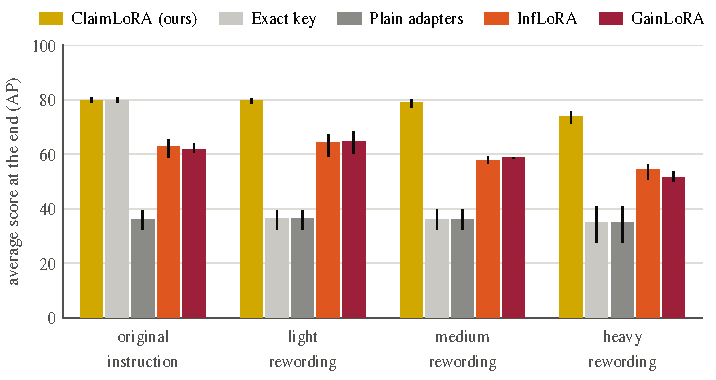
\includegraphics[width=0.9\linewidth]{figures/five_wordings}
  \caption{Average score at the end (AP) on the five tasks, with the original instructions and
  three levels of rewording. Bars are means over seeds; where there are several seeds a black line spans the lowest and the highest.}
  \label{fig:fivewordings}
\end{figure}

\begin{table}[t]
  \caption{Routes on the five tasks: how many test inputs are certified, how many are given to
  their own task, and how many answers change, for the certified switch and for the nearest-centre
  rule. Routes do not depend on the seed; counts are summed over seeds.}
  \label{tab:fiveroutes}
  \centering
  \small
  \setlength{\tabcolsep}{4.5pt}
  \begin{tabular}{lcccccc}
    \toprule
    & & \multicolumn{3}{c}{\cert{}} & \multicolumn{2}{c}{\centre{}} \\
    \cmidrule(lr){3-5} \cmidrule(lr){6-7}
    Wording & Tasks & Certified inputs & \shortstack[c]{Sent to own\\task $\uparrow$} & \shortstack[c]{Answers\\changed $\downarrow$} & \shortstack[c]{Sent to own\\task $\uparrow$} & \shortstack[c]{Answers\\changed $\downarrow$} \\
    \midrule
    original & 5 & 1{,}500 of 1{,}500 & 100.0\% & 0 of 1{,}200 & 100.0\% & 0 of 1{,}200 \\
    light & 5 & 1{,}500 of 1{,}500 & 100.0\% & 0 of 1{,}200 & 100.0\% & 0 of 1{,}200 \\
    medium & 5 & 300 of 1{,}500 & 100.0\% & 0 of 1{,}200 & 99.2\% & 0 of 1{,}200 \\
    heavy & 5 & 294 of 1{,}500 & 93.8\% & 0 of 1{,}200 & 72.2\% & 171 of 1{,}200 \\
    \bottomrule
\end{tabular}

\end{table}

A benchmark input carries its task definition word for word, so any rule that recognises the
definition looks perfect. The test that separates the rules is to ask the same task in other
words. Table~\ref{tab:fivewordings} and Figure~\ref{fig:fivewordings} repeat the evaluation with the
three rewordings of each definition, and Table~\ref{tab:fiveroutes} shows where the inputs go.

\paragraph{No answer changes under any wording.} For the certified switch the number of changed answers is zero in every column.
With the light rewording this is again guaranteed, because all \FiveCertZoneOneLight{} inputs are
still certified (Table~\ref{tab:fiveroutes}). With the medium and the heavy rewording it is not
guaranteed: only \FiveCertZoneOneMedium{} and \FiveCertZoneOneHeavy{} of the \FiveCertInputsOne{}
inputs are inside a zone, and they belong to relation extraction, the task with the longest
instruction. The other inputs kept their answers because no later task came nearer to them than
the task they had been given to, which Proposition~\ref{prop:uncertified} permits but does not
promise. It also depends on the order of the tasks: in an order in which SST-2 is learned after
Sentiment140, 31 routes of heavily reworded inputs would change when SST-2 arrives
(Section~\ref{sec:orders}). The average
score falls from \FiveCertAP{} with the original instructions to \FiveCertAPLight{},
\FiveCertAPMedium{} and \FiveCertAPHeavy{}.

\paragraph{An exact key is a lookup table.} \keyswitch{} compares the opening token for token. With the original instructions
it is perfect. With the light rewording, which changes a few words, it recognises nothing, leaves
all adapters on and ends at \FiveKeyAPLight{}, exactly where \plain{} ends. It fails because an
input that it does not recognise gets every adapter. \nearest{} and \cert{} send such an input to
the nearest zone instead, and they score alike on this benchmark; the radius of the zones decides
which of these inputs also carry the guarantee.

\paragraph{The nearest centre of the whole input fails under heavy rewording.} \centre{}, the nearest-centre rule with the token weights of Eq.~\eqref{eq:weights}, gives only
\FiveCentreRightHeavy{}\% of the heavily reworded inputs to their own task. Its score is
\FiveCentreAPHeavy{} against \FiveCertAPHeavy{}, and \FiveCentreChangedHeavy{} of
\FiveCentreComparedHeavy{} answers change as later tasks arrive. The first version of \cert{}, which used the nearest centre
with all tokens weighted equally, did better on these five tasks (97.4\% to the right task with seed 42, against
\FiveCertRightHeavy{}\% for the final rule) and was replaced because it failed on the 15-task sequence (Appendix~\ref{app:history}).

\paragraph{The published methods under rewording.} The published methods have no recognition step that a rewording could break, and
their forgetting scores stay within a few points in every wording, although many answers change (Table~\ref{tab:fivemore} in the
appendix). Their scores are \FiveInfAP{}, \FiveInfAPLight{}, \FiveInfAPMedium{} and
\FiveInfAPHeavy{} for InfLoRA and \FiveGainAP{}, \FiveGainAPLight{}, \FiveGainAPMedium{} and
\FiveGainAPHeavy{} for GainLoRA. The number of answers that differ at the end is largest under
heavy rewording, \FiveInfChangedHeavy{} and \FiveGainChangedHeavy{} of \FiveInfComparedHeavy{}.

\paragraph{Where the loss under heavy rewording comes from.} Under heavy rewording the certified switch scores \FiveCertAPHeavy{} instead of
\FiveCertAP{}. None of the difference is forgetting. One part is that the adapters themselves answer
a differently worded instruction less well: right after each task is learned, with all adapters on
(\plain{}), which at that moment is the right set of adapters, the score is
\FivePlainLearnedHeavy{}. The other part is routing:
\FiveCertWrongHeavy{} of the \FiveCertInputsOne{} heavily reworded inputs are given to another task,
which brings \FivePlainLearnedHeavy{} down to \FiveCertLearnedHeavy{}. All of them are tweets of the
Sentiment140 task that are given to SST-2, the other sentiment task.

\begin{figure}[t]
  \centering
  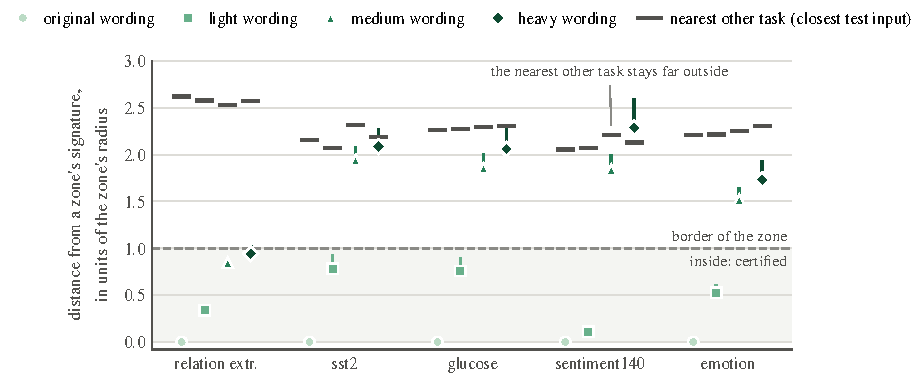
\includegraphics[width=0.92\linewidth]{figures/margins}
  \caption{Why rewording costs the certificate before it costs the route (five tasks, T5-base
  word-vectors). Markers: relative distance $\delta_k$ of the test inputs of a task from their own
  signature, in units of the radius of their own zone: median over the 100 inputs, with a line up to
  the farthest input. Short dark lines: how close the closest of these inputs comes to the signature of any
  \emph{other} task, in units of that task's radius. Below the dashed line an input is inside the
  zone, that is, certified.}
  \label{fig:margins}
\end{figure}

\paragraph{Where reworded inputs lie.}\label{sec:geometry} Figure~\ref{fig:margins} shows the geometry behind these numbers. With the original
wording every input lies exactly on the signature of its task (Proposition~\ref{prop:own}). The
light rewordings move the inputs by 0.1 to 0.8 radii, which is inside the zone. The medium and the
heavy rewordings move them by 1.5 to 2.3 radii in four of the five tasks, which is outside; relation
extraction, the task with the longest instruction, stays inside. The signatures of the other tasks,
however, are 2.1 to 2.6 of \emph{their} radii away from these inputs, so an input that has left its
zone is in most cases still nearer, in these units, to its own signature than to any other. The
certificate is lost long before the route is. The one place where the two margins cross is the
place of the errors: under the heavy rewording the tweets of Sentiment140 lie 2.29 radii from their
own signature (up to 2.60), and the signature of SST-2, the other sentiment task, is 2.13 of its
radii from the closest of them. Appendix~\ref{app:more} gives the numbers per task
(Table~\ref{tab:geometry}).

\subsection{Routes from the example alone: rewording cannot change the route}
\label{sec:exampleroutes}

The zones read the instruction, and a reworded instruction can leave them: under the heavy
rewording \cert{} sends some inputs to another task and ends below what the same adapters give
when every input reaches its own task (Section~\ref{sec:reworded}). \recog{} never
reads the instruction (Remark~\ref{rem:auditlimits}(v)). So the five tasks were trained once more
with their definitions (seed 42, plain adapters, nothing blocked), and the routes of \recog{} and
\handicap{} were computed from the example alone. It is the same route table as in the runs without
instructions (Section~\ref{sec:nodeftrained}), because these routes do not depend on the definition.
The scores of \cert{} equal those of the single-seed run of seed 42 with definitions, not those of the three-seed run of Table~\ref{tab:fivewordings} (seed 42 was trained twice; Section~\ref{sec:five}).
Line fixed before the run: \recog{} ``repairs the weak spot'' if its final score at the heavy
wording is at least 2 points above that of \cert{}, its score at the original wording is within
2 points of \cert{}, and at most 8 of the \AudUCompared{} compared answers change at every wording;
it ``does not'' if the heavy score is below that of \cert{} or the original score more than 4
points below.

\begin{table}[t]
  \caption{The five tasks with their definitions, seed 42, T5-base, 10 epochs, plain adapters; the
  same adapters under each rule, at the four wordings of the definition. Top: final score (AP,
  re-test). Bottom: answers to the test inputs of the first four tasks that differ at the end from
  the answer right after their task was learned, of \AudUCompared{}. \recog{} and \handicap{} set
  the route from the example alone; ``zone first'' uses the certified route where the input is
  inside a zone and the route of \recog{} or \handicap{} elsewhere. The rows of the published
  methods are from the run of the same seed in Section~\ref{sec:reworded}.}
  \label{tab:instanceroutes}
  \centering
  {\scriptsize\setlength{\tabcolsep}{2pt}\begin{tabular}{p{1.2in}rrrrrrrrr}
    \toprule
    & \multicolumn{4}{c}{Final score $\uparrow$} & \multicolumn{4}{c}{\shortstack{Answers changed\\of \AudUCompared{} $\downarrow$}} & \shortstack[r]{Sent to own\\task, heavy, \% $\uparrow$} \\
    \cmidrule(lr){2-5}\cmidrule(lr){6-9}
    & original & light & medium & heavy & original & light & medium & heavy & \\
    \midrule
    \cert{} (zones on the instruction) & \AudUOriginalCertAP{} & \AudULightCertAP{} & \AudUMediumCertAP{} & \AudUHeavyCertAP{} & \AudUOriginalCertChanged{} & \AudULightCertChanged{} & \AudUMediumCertChanged{} & \AudUHeavyCertChanged{} & \AudUHeavyCertRight{} \\
    \recog{} (example alone) & \AudUOriginalRidgeAP{} & \AudULightRidgeAP{} & \AudUMediumRidgeAP{} & \AudUHeavyRidgeAP{} & \AudUOriginalRidgeChanged{} & \AudULightRidgeChanged{} & \AudUMediumRidgeChanged{} & \AudUHeavyRidgeChanged{} & \AudUHeavyRidgeRight{} \\
    \handicap{}, $\nu = 2$ (example alone) & \AudUOriginalHandicapAP{} & \AudULightHandicapAP{} & \AudUMediumHandicapAP{} & \AudUHeavyHandicapAP{} & \AudUOriginalHandicapChanged{} & \AudULightHandicapChanged{} & \AudUMediumHandicapChanged{} & \AudUHeavyHandicapChanged{} & \AudUHeavyHandicapRight{} \\
    every input to its own task (ceiling) & \AudUOriginalOwnAP{} & \AudULightOwnAP{} & \AudUMediumOwnAP{} & \AudUHeavyOwnAP{} & \AudUOriginalOwnChanged{} & \AudULightOwnChanged{} & \AudUMediumOwnChanged{} & \AudUHeavyOwnChanged{} & \AudUHeavyOwnRight{} \\
    zone first, else \recog{} & \AudUOriginalMixRidgeAP{} & \AudULightMixRidgeAP{} & \AudUMediumMixRidgeAP{} & \AudUHeavyMixRidgeAP{} & \AudUOriginalMixRidgeChanged{} & \AudULightMixRidgeChanged{} & \AudUMediumMixRidgeChanged{} & \AudUHeavyMixRidgeChanged{} & \AudUHeavyMixRidgeRight{} \\
    zone first, else \handicap{} & \AudUOriginalMixHandicapAP{} & \AudULightMixHandicapAP{} & \AudUMediumMixHandicapAP{} & \AudUHeavyMixHandicapAP{} & \AudUOriginalMixHandicapChanged{} & \AudULightMixHandicapChanged{} & \AudUMediumMixHandicapChanged{} & \AudUHeavyMixHandicapChanged{} & \AudUHeavyMixHandicapRight{} \\
    \centre{} & \AudUOriginalCentreAP{} & \AudULightCentreAP{} & \AudUMediumCentreAP{} & \AudUHeavyCentreAP{} & \AudUOriginalCentreChanged{} & \AudULightCentreChanged{} & \AudUMediumCentreChanged{} & \AudUHeavyCentreChanged{} & \AudUHeavyCentreRight{} \\
    \plain{} & \AudUOriginalPlainAP{} & \AudULightPlainAP{} & \AudUMediumPlainAP{} & \AudUHeavyPlainAP{} & \AudUOriginalPlainChanged{} & \AudULightPlainChanged{} & \AudUMediumPlainChanged{} & \AudUHeavyPlainChanged{} & \AudUHeavyPlainRight{} \\
    \midrule
    GainLoRA & \AudWordOriginalGainloraAP{} & \AudWordLightGainloraAP{} & \AudWordMediumGainloraAP{} & \AudWordHeavyGainloraAP{} & \AudWordOriginalGainloraChanged{} & \AudWordLightGainloraChanged{} & \AudWordMediumGainloraChanged{} & \AudWordHeavyGainloraChanged{} & -- \\
    InfLoRA & \AudWordOriginalInfloraAP{} & \AudWordLightInfloraAP{} & \AudWordMediumInfloraAP{} & \AudWordHeavyInfloraAP{} & \AudWordOriginalInfloraChanged{} & \AudWordLightInfloraChanged{} & \AudWordMediumInfloraChanged{} & \AudWordHeavyInfloraChanged{} & -- \\
    \bottomrule
\end{tabular}}

\end{table}

Table~\ref{tab:instanceroutes} gives the result. At the heavy wording \recog{} ends at
\AudUHeavyRidgeAP{} and \handicap{} at \AudUHeavyHandicapAP{}, against \AudUHeavyCertAP{} for
\cert{} (seed 42; the mean over three seeds in Section~\ref{sec:reworded} is \FiveCertAPHeavy{});
the ceiling, with every input at its own task, is \AudUHeavyOwnAP{}. At the original
wording \recog{} ends at \AudUOriginalRidgeAP{} and \handicap{} at \AudUOriginalHandicapAP{},
against \AudUOriginalCertAP{}. At every wording \AudUOriginalRidgeChanged{} of \AudUCompared{}
answers change under \recog{} and \AudUOriginalHandicapChanged{} under \handicap{}, where \cert{}
changes none. All three lines hold: the verdict is ``repairs the weak spot''.
Our guesses (78.5 to 79.3 at the original wording, 75.5 to 76.7 at the heavy one) held, and one
was wrong in the good direction: we had expected about six changed answers for \recog{}, as in
the run without definitions. Six routes do change, but for three
of these inputs the model gives the same answer with the adapters up to either task. Without
definitions all six answers changed; why fewer change with the definition we did not test.

What this shows: the routes of \recog{} are the same at every wording, so its score stays
\AudURidgeBelowOwnLow{} to \AudURidgeBelowOwnHigh{} points below the ceiling at every wording
(\handicap{}: \AudUHandicapBelowOwnLow{} to \AudUHandicapBelowOwnHigh{} points), and what is lost
under rewording is what the adapters themselves lose when their instruction is reworded, not
misrouting. The zones are exact where the instruction is unedited and lose
\AudUHeavyCertBelowOwn{} points at the heavy wording through misrouted
inputs. The mixed rule has the best of both at the original, the light and the heavy wording; at
the medium wording it is below \cert{} (\AudUMediumMixRidgeAP{} and \AudUMediumMixHandicapAP{}
against \AudUMediumCertAP{}), whose own fallback is right for every input there. The published
methods end at \AudWordHeavyGainloraAP{} (GainLoRA) and \AudWordHeavyInfloraAP{} (InfLoRA) at the
heavy wording, with \AudWordHeavyGainloraChanged{} and \AudWordHeavyInfloraChanged{} changed
answers. This first run is one seed, five tasks, and three machine-written rewordings per task
that were looked at during development (Section~\ref{sec:protocol}), not
rewordings by people. Remark~\ref{rem:auditlimits}(v) says what this assumes about
the input.

\paragraph{Three seeds.} An independent reading of this result pointed out that seed 42 is the seed in which \cert{} loses most at the heavy wording. So the run was repeated for seeds 43 and 44 (Table~\ref{tab:instanceroutesseeds}).
Line fixed before these runs, for the means over the three seeds: the result ``stands for three seeds'' if the heavy score of \recog{} is at least 2 points above that of \cert{}, the original score is within 2 points of \cert{}, and in every seed at most 8 of \AudUCompared{} answers change at every wording.
It stands. At the heavy wording \recog{} ends at \AudUThreeHeavyRidgeAP{} and \handicap{} at \AudUThreeHeavyHandicapAP{}, against \AudUThreeHeavyCertAP{} for \cert{}, a gain of \AudUThreeHeavyRidgeAboveCert{} points; the ceiling is \AudUThreeHeavyOwnAP{}.
At the original wording \recog{} ends at \AudUThreeOriginalRidgeAP{}, \AudUThreeOriginalRidgeBelowCert{} points below \cert{} (\AudUThreeOriginalCertAP{}).
In no seed and at no wording do more than \AudUThreeMaxChangedPerSeed{} of \AudUCompared{} answers change under \recog{}.
Over the four wordings \recog{} stays \AudUThreeRidgeBelowOwnLow{} to \AudUThreeRidgeBelowOwnHigh{} points below the ceiling and \handicap{} \AudUThreeHandicapBelowOwnLow{} to \AudUThreeHandicapBelowOwnHigh{}; \cert{} loses \AudUThreeHeavyCertBelowOwn{} points at the heavy wording through misrouted inputs.
We had expected a smaller gain, 2 to 2.5 points: in seeds 43 and 44 the adapters themselves lose less under the heavy rewording than in seed 42.
These three seeds are not the training runs of Table~\ref{tab:fivewordings}: seed 42 is the single-seed run, and seeds 43 and 44 were trained again. So \cert{} ends at \AudUThreeOriginalCertAPOne{} (original) and \AudUThreeHeavyCertAPOne{} (heavy) here, and at \FiveCertAP{} and \FiveCertAPHeavy{} in Table~\ref{tab:fivewordings}; the difference is of the size seen between two runs of the same seed.
It remains five tasks, with machine-written rewordings that were looked at during development.

\begin{table}[t]
  \caption{As Table~\ref{tab:instanceroutes}, means over \AudUThreeSeeds{} seeds (42, 43, 44); changed answers are summed over the seeds. Training runs: seed 42 as in Table~\ref{tab:instanceroutes}, seeds 43 and 44 trained for this table; they are not the runs of Table~\ref{tab:fivewordings}, so the rows of \cert{} differ from it by a few tenths of a point.}
  \label{tab:instanceroutesseeds}
  \centering
  {\scriptsize\setlength{\tabcolsep}{2pt}\begin{tabular}{p{1.2in}rrrrrrrrr}
    \toprule
    & \multicolumn{4}{c}{Final score $\uparrow$} & \multicolumn{4}{c}{\shortstack{Answers changed\\of \AudUThreeCompared{} $\downarrow$}} & \shortstack[r]{Sent to own\\task, heavy, \% $\uparrow$} \\
    \cmidrule(lr){2-5}\cmidrule(lr){6-9}
    & original & light & medium & heavy & original & light & medium & heavy & \\
    \midrule
    \cert{} (zones on the instruction) & \AudUThreeOriginalCertAP{} & \AudUThreeLightCertAP{} & \AudUThreeMediumCertAP{} & \AudUThreeHeavyCertAP{} & \AudUThreeOriginalCertChanged{} & \AudUThreeLightCertChanged{} & \AudUThreeMediumCertChanged{} & \AudUThreeHeavyCertChanged{} & \AudUThreeHeavyCertRight{} \\
    \recog{} (example alone) & \AudUThreeOriginalRidgeAP{} & \AudUThreeLightRidgeAP{} & \AudUThreeMediumRidgeAP{} & \AudUThreeHeavyRidgeAP{} & \AudUThreeOriginalRidgeChanged{} & \AudUThreeLightRidgeChanged{} & \AudUThreeMediumRidgeChanged{} & \AudUThreeHeavyRidgeChanged{} & \AudUThreeHeavyRidgeRight{} \\
    \handicap{}, $\nu = 2$ (example alone) & \AudUThreeOriginalHandicapAP{} & \AudUThreeLightHandicapAP{} & \AudUThreeMediumHandicapAP{} & \AudUThreeHeavyHandicapAP{} & \AudUThreeOriginalHandicapChanged{} & \AudUThreeLightHandicapChanged{} & \AudUThreeMediumHandicapChanged{} & \AudUThreeHeavyHandicapChanged{} & \AudUThreeHeavyHandicapRight{} \\
    every input to its own task (ceiling) & \AudUThreeOriginalOwnAP{} & \AudUThreeLightOwnAP{} & \AudUThreeMediumOwnAP{} & \AudUThreeHeavyOwnAP{} & \AudUThreeOriginalOwnChanged{} & \AudUThreeLightOwnChanged{} & \AudUThreeMediumOwnChanged{} & \AudUThreeHeavyOwnChanged{} & \AudUThreeHeavyOwnRight{} \\
    zone first, else \recog{} & \AudUThreeOriginalMixRidgeAP{} & \AudUThreeLightMixRidgeAP{} & \AudUThreeMediumMixRidgeAP{} & \AudUThreeHeavyMixRidgeAP{} & \AudUThreeOriginalMixRidgeChanged{} & \AudUThreeLightMixRidgeChanged{} & \AudUThreeMediumMixRidgeChanged{} & \AudUThreeHeavyMixRidgeChanged{} & \AudUThreeHeavyMixRidgeRight{} \\
    zone first, else \handicap{} & \AudUThreeOriginalMixHandicapAP{} & \AudUThreeLightMixHandicapAP{} & \AudUThreeMediumMixHandicapAP{} & \AudUThreeHeavyMixHandicapAP{} & \AudUThreeOriginalMixHandicapChanged{} & \AudUThreeLightMixHandicapChanged{} & \AudUThreeMediumMixHandicapChanged{} & \AudUThreeHeavyMixHandicapChanged{} & \AudUThreeHeavyMixHandicapRight{} \\
    \centre{} & \AudUThreeOriginalCentreAP{} & \AudUThreeLightCentreAP{} & \AudUThreeMediumCentreAP{} & \AudUThreeHeavyCentreAP{} & \AudUThreeOriginalCentreChanged{} & \AudUThreeLightCentreChanged{} & \AudUThreeMediumCentreChanged{} & \AudUThreeHeavyCentreChanged{} & \AudUThreeHeavyCentreRight{} \\
    \plain{} & \AudUThreeOriginalPlainAP{} & \AudUThreeLightPlainAP{} & \AudUThreeMediumPlainAP{} & \AudUThreeHeavyPlainAP{} & \AudUThreeOriginalPlainChanged{} & \AudUThreeLightPlainChanged{} & \AudUThreeMediumPlainChanged{} & \AudUThreeHeavyPlainChanged{} & \AudUThreeHeavyPlainRight{} \\
    \midrule
    GainLoRA & \AudUThreeOriginalGainloraAP{} & \AudUThreeLightGainloraAP{} & \AudUThreeMediumGainloraAP{} & \AudUThreeHeavyGainloraAP{} & \AudUThreeOriginalGainloraChanged{} & \AudUThreeLightGainloraChanged{} & \AudUThreeMediumGainloraChanged{} & \AudUThreeHeavyGainloraChanged{} & -- \\
    InfLoRA & \AudUThreeOriginalInfloraAP{} & \AudUThreeLightInfloraAP{} & \AudUThreeMediumInfloraAP{} & \AudUThreeHeavyInfloraAP{} & \AudUThreeOriginalInfloraChanged{} & \AudUThreeLightInfloraChanged{} & \AudUThreeMediumInfloraChanged{} & \AudUThreeHeavyInfloraChanged{} & -- \\
    \bottomrule
\end{tabular}}

\end{table}
